\documentclass[aspectratio=169]{beamer} % Формат 16:9

\usepackage[T2A]{fontenc}
\usepackage[utf8]{inputenc}
\usepackage[russian]{babel}
\usepackage{cmap}
\usepackage{graphicx}
\usepackage{xspace}
\usepackage{psfrag}
\usepackage{hyperref}
\usepackage[normalem]{ulem}
\usepackage[table]{xcolor} % Для цветных ячеек в таблицах

\beamertemplatenavigationsymbolsempty
\setbeamertemplate{footline}[frame number]
\usecolortheme{seahorse}

% Цвет для заголовков таблиц из вашей презентации
\definecolor{tabgreen}{HTML}{92D050}

%%Исправляем греческие буквы в формулах
\DeclareSymbolFont{greek}{U}{eur}{m}{n}                                                        
\SetSymbolFont{greek}{bold}{U}{eur}{b}{n}                                                      
\DeclareSymbolFontAlphabet{\gr}{greek}                                                         
\DeclareMathSymbol{\alpha}{\mathord}{greek}{"0B}                                               
\DeclareMathSymbol{\beta}{\mathord}{greek}{"0C}                                                
\DeclareMathSymbol{\gamma}{\mathord}{greek}{"0D}                                               
\DeclareMathSymbol{\delta}{\mathord}{greek}{"0E}                                               
\DeclareMathSymbol{\epsilon}{\mathord}{greek}{"0F}                                             
\DeclareMathSymbol{\zeta}{\mathord}{greek}{"10}                                                
\DeclareMathSymbol{\eta}{\mathord}{greek}{"11}                                                 
\DeclareMathSymbol{\theta}{\mathord}{greek}{"12}                                               
\DeclareMathSymbol{\iota}{\mathord}{greek}{"13}                                                
\DeclareMathSymbol{\kappa}{\mathord}{greek}{"14}                                               
\DeclareMathSymbol{\lambda}{\mathord}{greek}{"15}                                              
\DeclareMathSymbol{\mu}{\mathord}{greek}{"16}                                                  
\DeclareMathSymbol{\nu}{\mathord}{greek}{"17}                                                  
\DeclareMathSymbol{\xi}{\mathord}{greek}{"18}                                                  
\DeclareMathSymbol{\pi}{\mathord}{greek}{"19}                                                  
\DeclareMathSymbol{\rho}{\mathord}{greek}{"1A}                                                 
\DeclareMathSymbol{\sigma}{\mathord}{greek}{"1B}                                               
\DeclareMathSymbol{\tau}{\mathord}{greek}{"1C}                                                 
\DeclareMathSymbol{\upsilon}{\mathord}{greek}{"1D}                                             
\DeclareMathSymbol{\phi}{\mathord}{greek}{"1E}                                                 
\DeclareMathSymbol{\chi}{\mathord}{greek}{"1F}                                                 
\DeclareMathSymbol{\psi}{\mathord}{greek}{"20}                                                 
\DeclareMathSymbol{\omega}{\mathord}{greek}{"21}                                               
\DeclareMathSymbol{\varepsilon}{\mathord}{greek}{"22}                                          
\DeclareMathSymbol{\vartheta}{\mathord}{greek}{"23}                                            
\DeclareMathSymbol{\varpi}{\mathord}{greek}{"24}                                               
\let\varrho\rho                                                                                
\let\varsigma\sigma                                                                            
\DeclareMathSymbol{\varphi}{\mathord}{greek}{"27}

% Настройка титульного листа
\title{Создание интеллектуальных ассистентов для инженерных продуктов на примере узкоспециализированных предметных областей}
\author{%
  \begin{tabular}{rl}
    Студент: & Михайлов Николай Кириллович, 932302 \\[0.3cm]
    Научный руководитель: & к.т.н. Пожидаев Михаил Сергеевич
  \end{tabular}
}
\date{} 

\begin{document}

% --- Слайд 1 ---
\begin{frame}
\maketitle
\end{frame}

% --- Слайд 2 ---
\begin{frame}
\frametitle{Объект и предмет исследования}
\textbf{Объект исследования:} извлечение и генерация информации с использованием больших языковых моделей (LLM) и технологий дополненного поиска \\[0.5cm]
\textbf{Предмет исследования:} архитектурные методы и алгоритмические стратегии, определяющие точность и полноту извлечения знаний в RAG-системах
\end{frame}

% --- Слайд 3 ---
\begin{frame}
\frametitle{Цель исследования}
Создание RAG-системы, обеспечивающей высокую достоверность и минимизацию информационного шума при работе с документацией программных продуктов для узкоспециализированных предметных областей
\end{frame}

% --- Слайд 4 (Картинка 1) ---
\begin{frame}
\frametitle{Актуальность}
\begin{figure}[h]
    \centering
    % Положите файл scheme4.png в папку с проектом
    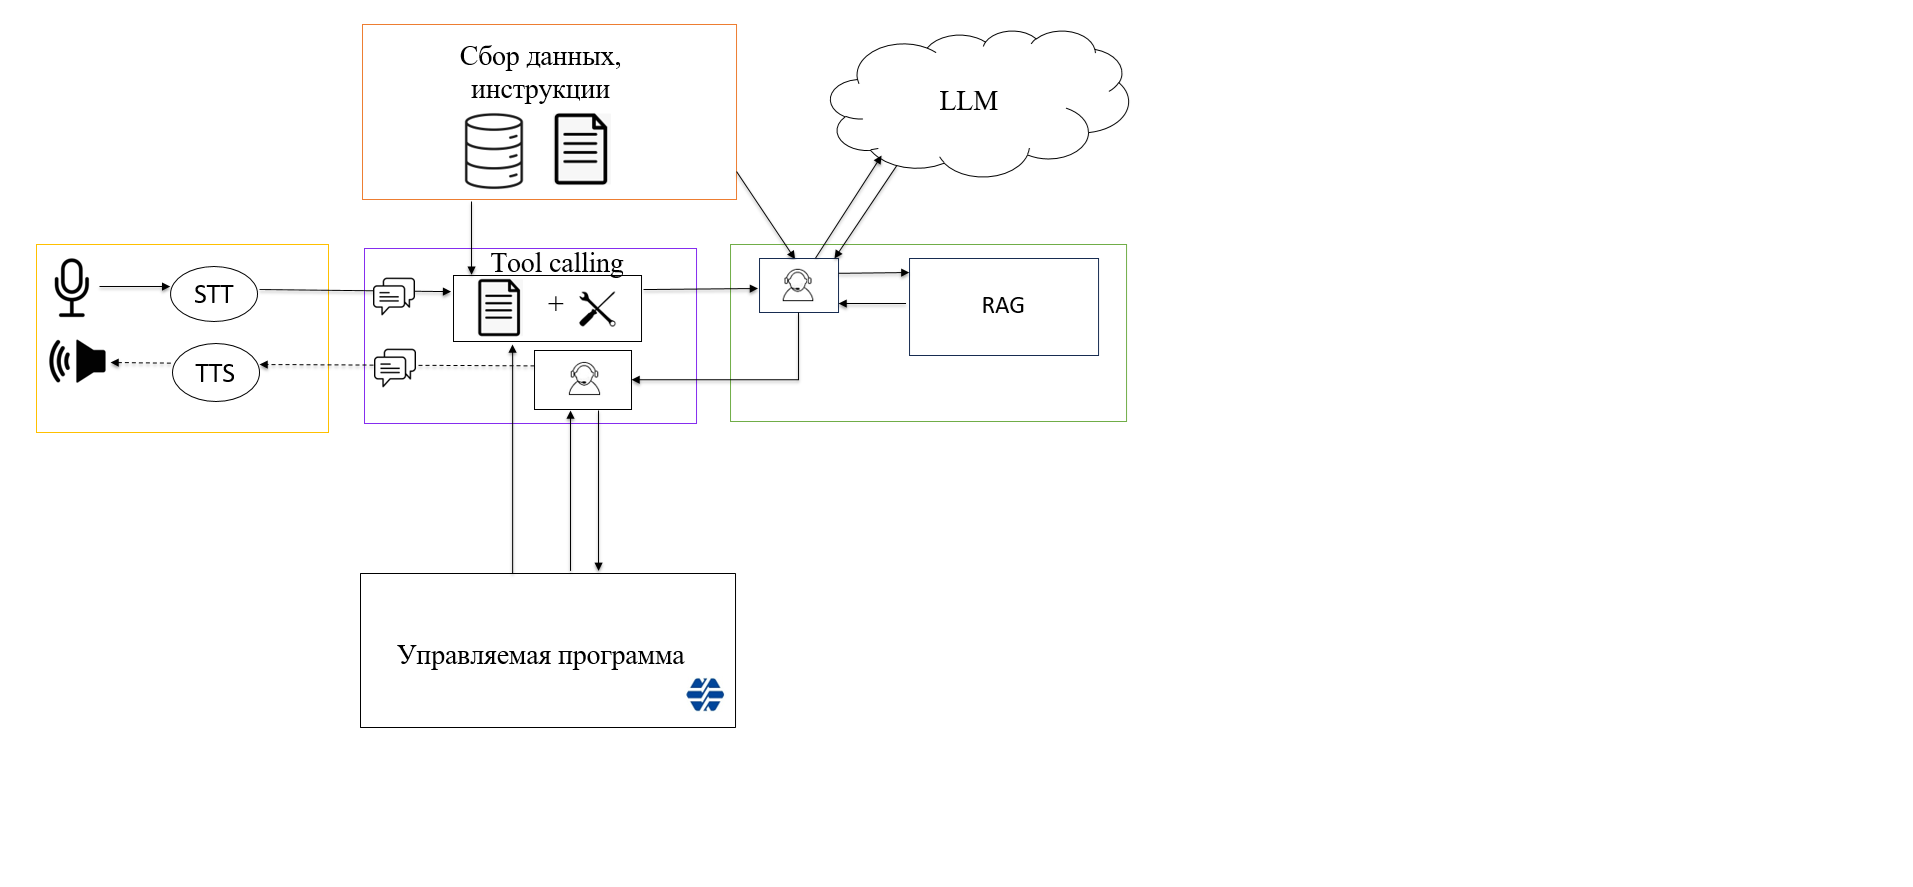
\includegraphics[width=0.9\textwidth, height=0.7\textheight, keepaspectratio]{scheme4.png}
\end{figure}
\end{frame}

% --- Слайд 5 (Картинка 2) ---
\begin{frame}
\frametitle{Актуальность}
\begin{figure}[h]
    \centering
    % Положите файл scheme5.png в папку с проектом
    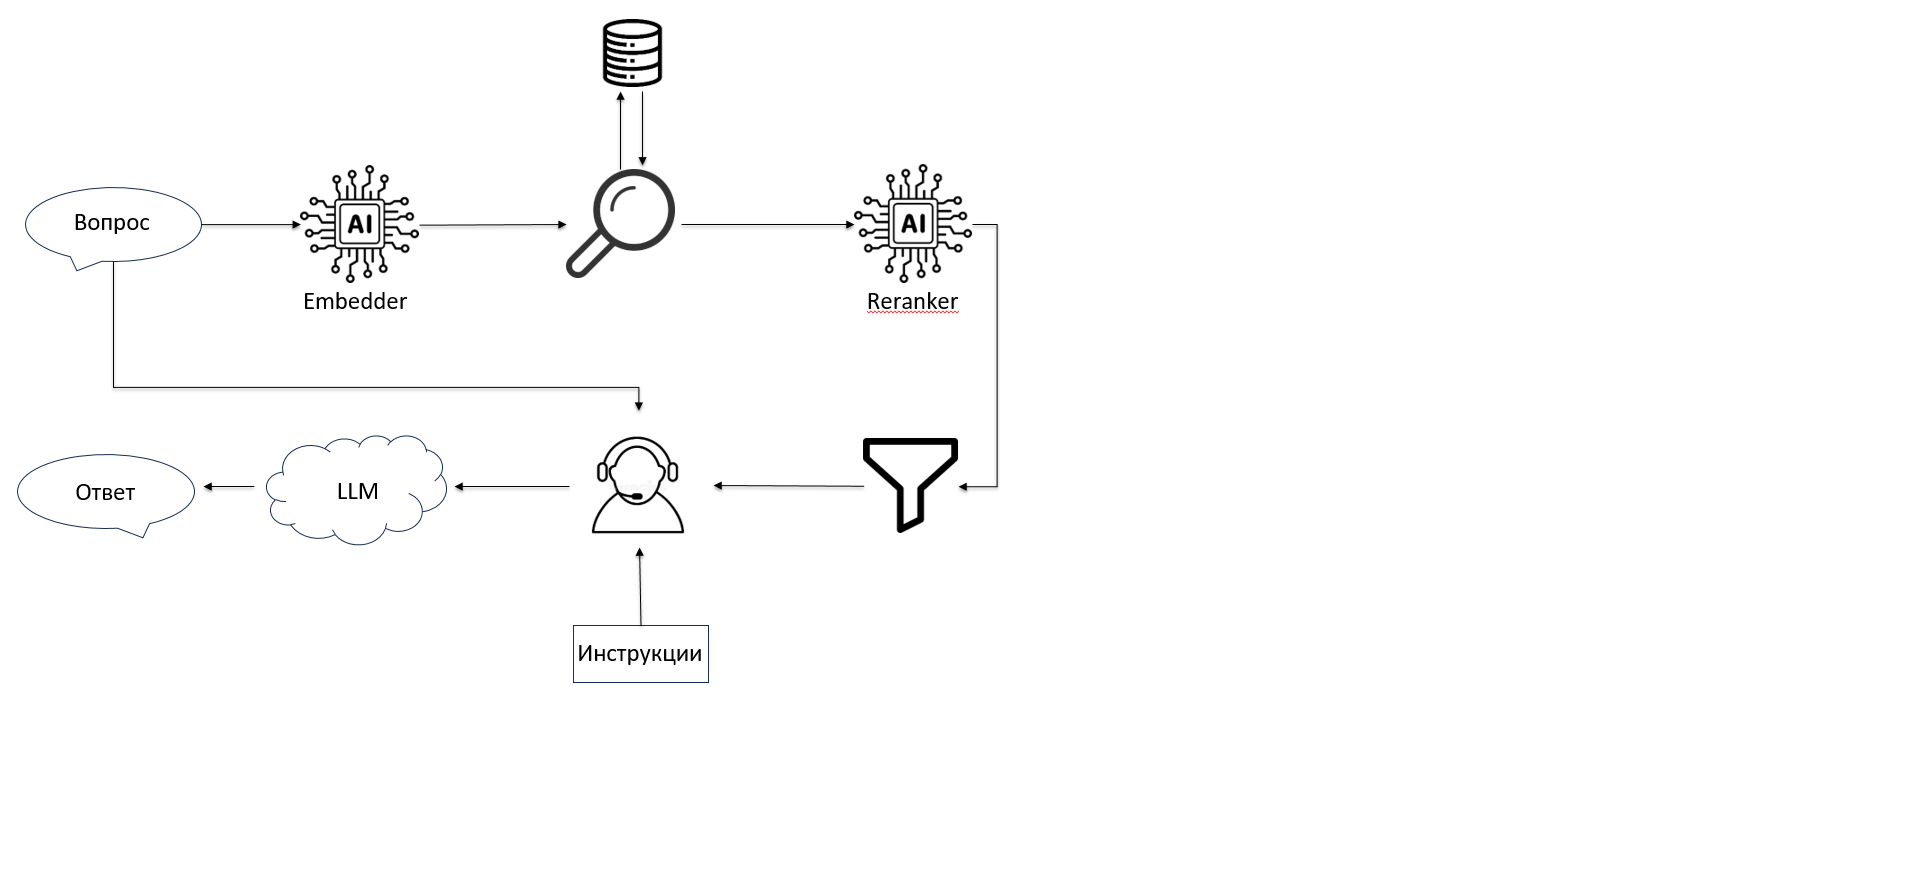
\includegraphics[width=0.9\textwidth, height=0.7\textheight, keepaspectratio]{scheme5.png}
\end{figure}
\end{frame}

% --- Слайд 6 ---
\begin{frame}
\frametitle{Задачи}
\small
\begin{enumerate}
    \item Провести теоретический анализ существующих поколений архитектур RAG.
    \item Адаптировать и локализовать методику автоматизированной оценки RAGAS.
    \item Разработать стратегию специализированной предобработки данных, включающую иерархическую нарезку текста, для сохранения логической структуры инженерной документации.
    \item Реализовать модуль семантической оптимизации запросов.
    \item Спроектировать механизм глобального гибридного поиска.
    \item Провести сравнительный анализ эффективности различных LLM.
    \item Провести сравнительное тестирование современных моделей векторных представлений.
    \item Интегрировать механизмы заключительной обработки.
\end{enumerate}
\end{frame}

% --- Слайд 7 ---
\begin{frame}
\frametitle{Эволюция архитектурных подходов RAG}
\begin{itemize}
    \item \textbf{Naive RAG:} прямой поиск и генерация
    \item \textbf{Advanced RAG:} введение предобработки запроса и обработки найденного контекста
    \item \textbf{Modular RAG:} гибкая перестановка модулей и итеративный поиск
\end{itemize}
\end{frame}

% --- Слайд 8 ---
\begin{frame}
\frametitle{Автоматизированная оценка с использованием фреймворка RAGAS}
\begin{itemize}
    \item Faithfulness (достоверность)
    \item Answer Accuracy (точность ответа)
    \item Context Precision (точность контекста)
    \item Context Recall (полнота контекста)
\end{itemize}
\end{frame}

% --- Слайд 9 ---
\begin{frame}
\frametitle{Стратегия специализированной предобработки}
\textbf{Проблема:} потеря структуры заголовков при обычном разбиении \\[0.5cm]
\textbf{Решение:} сохранение метаданных о структуре документа
\end{frame}

% --- Слайд 10 ---
\begin{frame}
\frametitle{Модуль трансформации пользовательских запросов}
\begin{itemize}
    \item \textbf{Query Expansion:} генерация нескольких вариантов запроса синонимичных исходному
    \item \textbf{HyDE:} создание гипотетического ответа для улучшения векторного поиска
\end{itemize}
\end{frame}

% --- Слайд 11 ---
\begin{frame}
\frametitle{Гибридный поиск}
\begin{itemize}
    \item \textbf{Dense Retrieval:} поиск по смыслу
    \item \textbf{Sparse Retrieval:} поиск по точным терминам
    \item \textbf{Метод объединения:} Reciprocal Rank Fusion
\end{itemize}
\end{frame}

% --- Слайд 12 ---
\begin{frame}
\frametitle{Условия проведения тестирования}
Тестирование системы проводилось на базе вопросов пользователей программных продуктов компании <<ИндорСофт>> и обучающей документации на официальном сайте той же компании.
\end{frame}

% --- Слайд 13 ---
\begin{frame}
\frametitle{Тестирование эмбеддеров}
\centering
\renewcommand{\arraystretch}{1.3} % Увеличиваем высоту строк для красоты
\begin{tabular}{|l|c|c|c|c|}
    \hline
    \rowcolor{tabgreen} \textbf{Модель} & \textbf{Faithfulness} & \textbf{Context recall} & \textbf{Context precision} & \textbf{Answer accuracy} \\ \hline
    BGE-M3 & 0,76 & 0,63 & 0,30 & 0,60 \\ \hline
    mGTE & 0,73 & 0,63 & 0,29 & 0,59 \\ \hline
    E5 + Splade & 0,53 & 0,40 & 0,14 & 0,36 \\ \hline
    E5 + BM25 & 0,74 & 0,63 & 0,34 & 0,59 \\ \hline
    RuBGE & 0,61 & 0,52 & 0,24 & 0,57 \\ \hline
    Fasttext (FB) + BM25 & 0,54 & 0,46 & 0,20 & 0,52 \\ \hline
    Fasttext (RV) + BM25 & 0,59 & 0,42 & 0,21 & 0,51 \\ \hline
\end{tabular}
\end{frame}

% --- Слайд 14 ---
\begin{frame}
\frametitle{Сравнение языковых моделей в роли генератора}
\centering
\renewcommand{\arraystretch}{1.5}
\begin{tabular}{|p{5cm}|p{3cm}|}
    \hline
    \rowcolor{tabgreen} \textbf{Модель} & \textbf{Faithfulness} \\ \hline
    Qwen-4b-instruct & 0,59 \\ \hline
    gpt-oss-20b & 0,76 \\ \hline
    Deepseek v3.2 & 0,87 \\ \hline
\end{tabular}
\end{frame}

% --- Слайд 15 ---
\begin{frame}
\frametitle{Оптимизация результатов: Reranking}
\centering
\renewcommand{\arraystretch}{1.5}
\begin{tabular}{|l|c|c|c|c|}
    \hline
    \rowcolor{tabgreen} \textbf{Модель} & \textbf{Faithfulness} & \textbf{Context recall} & \textbf{Context precision} & \textbf{Answer accuracy} \\ \hline
    BGE-M3 & 0,76 & 0,63 & 0,30 & 0,60 \\ \hline
    BGE-M3 + Reranker & 0,76 & 0,69 & 0,43 & 0,75 \\ \hline
\end{tabular}
\end{frame}

% --- Слайд 16 ---
\begin{frame}
\frametitle{Итоговая оценка оптимизированной архитектуры}
\centering
\renewcommand{\arraystretch}{1.3}
\small
\begin{tabular}{|p{4.5cm}|c|c|c|c|}
    \hline
    \rowcolor{tabgreen} \textbf{Конфигурация} & \textbf{Faithfulness} & \textbf{Context recall} & \textbf{Context precision} & \textbf{Answer accuracy} \\ \hline
    Qwen-4b-instruct + BGE-M3 & 0,59 & 0,61 & 0,31 & 0,58 \\ \hline
    gpt-oss-20b + BGE-M3 & 0,76 & 0,63 & 0,30 & 0,60 \\ \hline
    gpt-oss-20b + BGE-M3 + Reranker & 0,76 & 0,69 & 0,46 & 0,75 \\ \hline
    gpt-oss-20b + BGE-M3 + Reranker + Rewriter & 0,77 & 0,76 & 0,52 & 0,77 \\ \hline
    Deepseek v3.2 + BGE-M3 + Reranker + Rewriter & 0,87 & 0,75 & 0,54 & 0,75 \\ \hline
\end{tabular}
\end{frame}

% --- Слайд 17 ---
\begin{frame}
\frametitle{Результаты}
\small
\begin{enumerate}
    \item Проведён теоретический анализ существующих поколений архитектур RAG.
    \item Адаптирована и локализована методика автоматизированной оценки RAGAS.
    \item Разработана стратегия специализированной предобработки данных, включающая иерархическую нарезку текста.
    \item Реализован модуль семантической оптимизации запросов.
    \item Реализован механизм глобального гибридного поиска.
    \item Проведён сравнительный анализ эффективности различных LLM.
    \item Проведено сравнительное тестирование современных моделей векторных представлений.
    \item Интегрированы механизмы заключительной обработки.
\end{enumerate}
\end{frame}

% --- Слайд 18 ---
\begin{frame}
\vspace{2cm}
\centering
\Huge \textbf{Спасибо за внимание!}
\end{frame}

\end{document}